\chapter{MixVRTの実装}\label{cha:Implementation}
本章では、試作した\toolName の実装について説明する。
% なお、本研究で用いる、\toolName の各処理部が取得または生成する画像名を、以下に定義する。
% \begin{itemize}
%     \item Webページの変更前画像
%     \item Webページの変更後画像
%     \item 高解像度にしたWebページの変更前画像
%     \item 高解像度にしたWebページの変更後画像
%     \item 画像比較に基づく削除箇所を赤枠で囲むことで強調表示した、Webページの変更前画像
%     \item 画像比較に基づく追加箇所を緑枠で囲むことで強調表示した、Webページの変更後画像
%     \item HTMLコードにおけるbody要素内の追加とstyle要素内の追加のどちらか、
%           または両方の追加による影響を受けた箇所を赤枠で囲むことで強調表示した、Webページの変更前画像
%     \item HTMLコードにおけるbody要素内の削除とstyle要素内の削除のどちらか、
%           または両方の削除による影響を受けた箇所を緑枠で囲むことで強調表示した、Webページの変更後画像
%     \item HTMLコードの変更に基づく影響箇所を色付きの枠で囲むことで強調表示した、Webページの変更前画像
%     \item HTMLコードの変更に基づく影響箇所を色付きの枠で囲むことで強調表示した、Webページの変更後画像
%     \item レイアウトの不具合箇所を色付きの枠で囲むことで強調表示した、Webページの変更前画像
%     \item レイアウトの不具合箇所を色付きの枠で囲むことで強調表示した、Webページの変更後画像
% \end{itemize}
\par
\toolName のシステム構成を、図\ref{fig:System}に示す。
\begin{figure}[tp]
    \begin{center}
        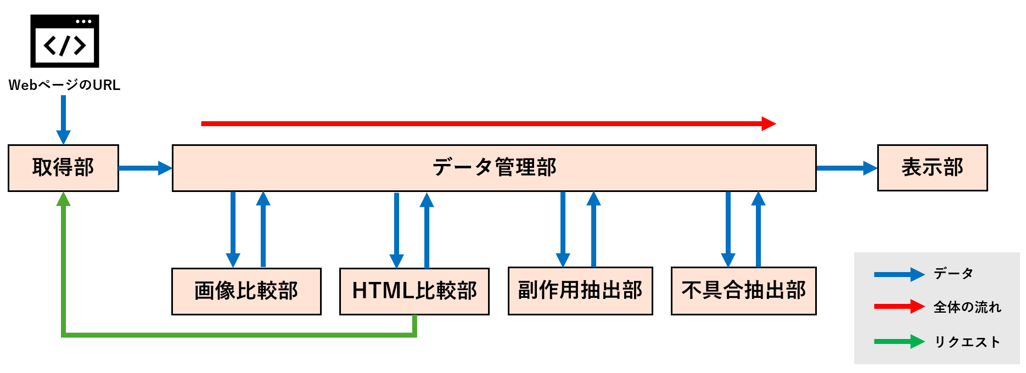
\includegraphics[width=1.0\columnwidth]{image/4_System_2.png}
        \caption{\toolName のシステム構成}
        \label{fig:System}
    \end{center}
\end{figure}
% 私の開発したツールは、まずユーザーがWebページのURLを入力します。
% このURLを受け取ると、ツールは該当するWebページから画像を取得し、
% これらの画像に対して特定の処理を行います。処理された画像は"static/images"ディレクトリに保存されます。
% そして、Flaskがローカルサーバを提供し、
% "templates"フォルダにあるHTMLコードが"static/images"ディレクトリを参照できるようになっています。
% この仕組みにより、ユーザーはローカルに立てられたFlaskサーバを通じて、
% Webページ上で生成された画像を確認することができます。
\toolName は、以下の7つの処理部から構成する。
\begin{itemize}
    \item データ管理部
    \item 取得部
    \item 画像比較部
    \item HTML比較部
    \item 副作用抽出部
    \item 不具合抽出部
    \item 表示部
          % \item 表示部
\end{itemize}
% \begin{itemize}
%     \item 取得部
%     \item 画像比較部
%           \begin{enumerate}
%               \item 差分箇所検出
%           \end{enumerate}
%     \item HTML比較部
%           \begin{enumerate}
%               \item 差分コード生成
%               \item 差分コード解析
%               \item 影響箇所強調HTMLコード生成
%           \end{enumerate}
%     \item レイアウト副作用箇所抽出部
%     \item 表示部
% \end{itemize}
以降、\toolName を構成する7つの処理部について説明する。
\par

\section{データ管理部}\label{sec:data_admin_section}
データ管理部は、システム内の各処理部間における、データの伝達を担い、他の処理部とのデータのやり取りとデータの保存を行う。
なお、本論文におけるデータとは、処理前後のWebページの画像やHTMLコードであり、
やり取りしたデータはデータ管理部が持つディレクトリに保存する。
また、取得部(\ref{sec:Web_data_get_section}節で後述)と表示部(\ref{sec:Interface_Display_Section}節で後述)のみ、データ管理部とのデータのやり取りが一方向である(図\ref{fig:System}を参照)。
% また、取得部とデータ管理部の間におけるデータのやり取りは、取得部からデータ管理部への一方向のみであり、
% データ管理部と表示部の間におけるデータのやり取りは、データ管理部から表示部への一方向のみである。
\par
データ管理部における最初のデータのやり取りは、取得部である。
取得部からデータを受け取ると、そのデータをデータ管理部のbase\_dirディレクトリに保存する。
保存した後、データがそれ以外に存在しない場合、全体の処理を終了する。
データがそれ以外に存在する場合、
画像比較部(\ref{sec:Difference_extraction_section}節で後述)、HTML比較部(\ref{sec:Affected_area_extraction}節で後述)、
副作用抽出部(\ref{sec:Layout_subEffect_extraction_section}節で後述)、不具合抽出部(\ref{sec:Layout_bug_extraction_section}節で後述)、表示部の順に
データのやり取りを行う。
データ管理部における最後のデータのやり取りは、表示部である。
表示部に出力するデータは、\ref{subsec:MixVRT_IO}節で述べた8つのPNG形式の画像のみである。
\par
各処理部との間でやり取りしたデータを保存する各ディレクトリを、以下に示す。
\begin{itemize}
    \item base\_dirディレクトリ:\\
          取得部で取得したWebページの画像とHTMLコードを保存する。
          %   \begin{itemize}
          %       \item currentディレクトリ:\\
          %             Webページの変更前画像と変更前HTMLコードを保存する。
          %       \item latestディレクトリ:\\
          %             Webページの変更後画像と変更後HTMLコードを保存する。
          %   \end{itemize}
    \item diff\_dirディレクトリ:\\
          画像比較部、HTML比較部、副作用抽出部、不具合抽出部でやり取りしたデータを保存する。
    \item disp\_dirディレクトリ:\\
          表示部に出力するデータを保存する。
          % Webページの変更前画像と変更後画像、Webページの変更前HTMLコードと変更後HTMLコードを用いて、
\end{itemize}
また、各ディレクトリに保存するデータの詳細を、以下の表に示す。
% \begin{table}[tp]
%     \caption{VariableHolder構造体が持つプロパティ}
%     \label{tb: VariableHolder}
%     \centering
%     \begin{tabular}{c|l}
%         \hline
%         プロパティ                 & \multicolumn{1}{c}{説明}   \\
%         \hline \hline
%         name                       & \begin{tabular}{l}プロパティの名前を保持する。\end{tabular}  \\ \hline
%         accessLevel                & \begin{tabular}{l}プロパティのアクセスレベルを保持する。\end{tabular}  \\ \hline
%         variableKind               & \begin{tabular}{l}型が表に示したケースのどれなのかを表す。\end{tabular}  \\ \hline
%         customAttribute            & \begin{tabular}{l}プロパティラッパの名前を保持する。\end{tabular}  \\ \hline
%         isStatic                   & \begin{tabular}{l}型プロパティの場合trueとなる。\end{tabular}  \\ \hline
%         isLazy                     & \begin{tabular}{l}遅延格納プロパティの場合trueとなる。\end{tabular}  \\ \hline
%         isConstant                 & \begin{tabular}{l}定数の場合trueとなる。\end{tabular} \\ \hline
%         literalType                & \begin{tabular}{l}型の種類がliteralの場合の型の名前を保持する。\end{tabular} \\ \hline
%         arrayType                  & \begin{tabular}{l}型の種類がarrayの場合の型の名前を保持する。\end{tabular} \\ \hline
%         dictionaryKeyType          & \begin{tabular}{l}型の種類がdictionaryの場合のキーの型の名前を保持する。\end{tabular} \\ \hline
%         dictionaryValueType        & \begin{tabular}{l}型の種類がdictionaryの場合のバリューの型の名前を保持する。\end{tabular} \\ \hline
%         tupleTypes                 & \begin{tabular}{l}型の種類がtupleの場合の型の名前を保持する。\end{tabular} \\ \hline
%         \begin{tabular}{l}conformedProtocol-\\ByOpaqueResultType\end{tabular} & \begin{tabular}{l}Opaque型が準拠するプロトコルの名前を保持する。\end{tabular} \\ \hline
%         isOptionalType             & \begin{tabular}{l}オプショナル型の場合trueとなる。\end{tabular} \\ \hline
%         initialValue               & \begin{tabular}{l}プロパティの初期値を保持する。\end{tabular} \\ \hline
%         haveWillSet                & \begin{tabular}{l}プロパティオブザーバのうちwillSetを持つ場合trueとなる。\end{tabular} \\ \hline
%         haveDidSet                 & \begin{tabular}{l}プロパティオブザーバのうちdidSetを持つ場合trueとなる。\end{tabular} \\ \hline
%         haveGetter                 & \begin{tabular}{l}getを持つ計算プロパティの場合trueとなる。\end{tabular} \\ \hline
%         haveSetter                 & \begin{tabular}{l}setを持つ計算プロパティの場合trueとなる。\end{tabular} \\ \hline
%     \end{tabular}
% \end{table}

% \toolName を2回実行した際の、データ管理部と各処理部とのやり取りを行ったデータを保存するディレクトリの構造を、以下に示す。

% % directory

% \begin{lstlisting}[language=, basicstyle=\ttfamily]
% .
% ├── base_dir/
% │   ├── (2回目実行時のタイムスタンプ)/
% │   │   ├── html/
% │   │   │   └── html_(2回目実行時のタイムスタンプ).html
% │   │   └── img/
% │   │       └── img_(2回目実行時のタイムスタンプ).png
% │   ├── current/ 
% │   │   ├── html/
% │   │   │   └── html_(1回目実行時のタイムスタンプ).html
% │   │   └── img/
% │   │       └── img_(1回目実行時のタイムスタンプ).png
% │   ├── initial/
% │   │   ├── html/
% │   │   │   └── html_(1回目実行時のタイムスタンプ).html
% │   │   └── img/
% │   │       └── img_(1回目実行時のタイムスタンプ).png
% │   └── latest/
% │       ├── html/
% │       │   └── html_(2回目実行時のタイムスタンプ).html
% │       └── img/
% │           └── img_(2回目実行時のタイムスタンプ).png
% └── diff_dir/
%      ├── diff_img_png/
%      │   ├── diff_af_img.png
%      │   └── diff_bf_img.png
%      ├── diff_rec_html_high_png/
%      │   ├── diff_rec_af_html.png
%      │   └── diff_rec_bf_html.png
%      ├── diff_rec_img_high_png/
%      │   ├── diff_rec_af_img.png
%      │   └── diff_rec_bf_img.png
%      ├── diff_html_txt/
%      │   └── diff_html.txt
%      ├── modified_html/
%      │   └── templates/
%      │       ├── modified_testPage_af.html
%      │       └── modified_testPage_bf.html
%      ├── modified_html_png/
%      │   ├── modified_testPage_af.png
%      │   └── modified_testPage_bf.png
%      ├── modifiled_html_high_png/
%      │   ├── modified_testPage_af_high.png
%      │   └── modified_testPage_bf_high.png
%      ├── original_high_png/
%      │   ├── img_af_high.png
%      │   └── img_bf_high.png
%      └── sub_effect_png/
%          ├── subEffect_af.png
%          └── subEffect_bf.png
% \end{lstlisting}

% \begin{itemize}
%     \item 取得部からデータ管理部
%     \item データ管理部から表示部
% \end{itemize}

% 5つの各処理部から受け付けるデータを、以下に示す。
% \begin{itemize}
%     \item 取得部:
%           \begin{itemize}
%               \item Webページの変更前画像と変更後画像
%           \end{itemize}
%     \item 画像比較部:
%           \begin{itemize}
%               \item 画像比較に基づく差分箇所を色付きの枠で囲むことで強調表示した、Webページの変更前画像と変更後画像
%               \item 上記の画像を高解像度にし、枠のみを抽出した、削除強調マスク画像と追加強調マスク画像
%           \end{itemize}
%     \item HTML比較部:
%           \begin{itemize}
%               \item HTMLコードの変更に基づく影響箇所を色付きの枠で囲むことで強調表示した、Webページの変更前画像と変更後画像
%               \item 上記の画像を高解像度にし、枠のみを抽出した、削除強調マスク画像と追加強調マスク画像
%           \end{itemize}
%     \item 副作用抽出部:
%           \begin{itemize}
%               \item レイアウトの副作用箇所を色付きの枠で囲むことで強調表示した、Webページの変更前画像と変更後画像
%           \end{itemize}
%     \item 不具合抽出部:
%           \begin{itemize}
%               \item レイアウトの不具合箇所を色付きの枠で囲むことで強調表示した、Webページの変更前画像と変更後画像
%           \end{itemize}
% \end{itemize}

% なお、\toolName の初回実行時は、取得部からWebページの画像とHTMLを受け取ると、\toolName 全体の処理を終了する。

\section{取得部}\label{sec:Web_data_get_section}
取得部は、テキスト端末上からWebページのURLを入力として受け取り、URLから取得したWebページの画像とHTMLコードを、データ管理部のbase\_dirディレクトリに出力する。
なお、HTML比較部から取得部に、枠付きWebページのURL(\ref{sec:Flask}節を参照)を与えて呼び出す場合があり(図\ref{fig:System}と\ref{sec:Affected_area_extraction}節を参照)、
その場合は、取得したデータをデータ管理部のdiff\_dirディレクトリに出力する。
\par
Webページの画像取得には、Selenium WebDriver(\ref{sec:Selenium_WebDriver}節を参照)を用いて、WebページのURLからWebページの画像を取得する。
なお、取得するWebページの画像は、フルページのスクリーンショット画像である。
WebページのHTMLコード取得には、Pythonライブラリの1つであるrequests(\ref{sec:requests}節を参照)を用いて、
WebページのURLからWebページのHTMLコードを取得する。

\section{画像比較部}\label{sec:Difference_extraction_section}
画像比較部は、データ管理部のbase\_dirディレクトリからWebページの変更前画像と変更後画像を受け取り、
画像比較に基づく差分箇所を色付きの枠で囲むことで強調表示した、Webページの変更前画像と変更後画像を生成する。
また、それらの画像から枠のみを残してそれ以外の部分を黒くすることで、差分箇所を囲む色付きの枠のみを抽出した、「差分箇所赤枠強調マスク画像」と「差分箇所緑枠強調マスク画像」も生成する。
生成した画像は、データ管理部のbase\_dirディレクトリに出力する。
\par
画像比較部の処理の流れを、以下に示す。
\begin{enumerate}
    \item 高解像度画像生成処理
    \item 適応的二値化処理
    \item 差分検出処理
    \item 膨張処理
    \item 輪郭検出処理
    \item 枠描画処理
\end{enumerate}
また、\toolName のテスト対象とするWebページの変更前画像と変更後画像の例を、図\ref{fig: img_original_bf_af}に示す。
\begin{figure}[tp]
    \begin{center}
        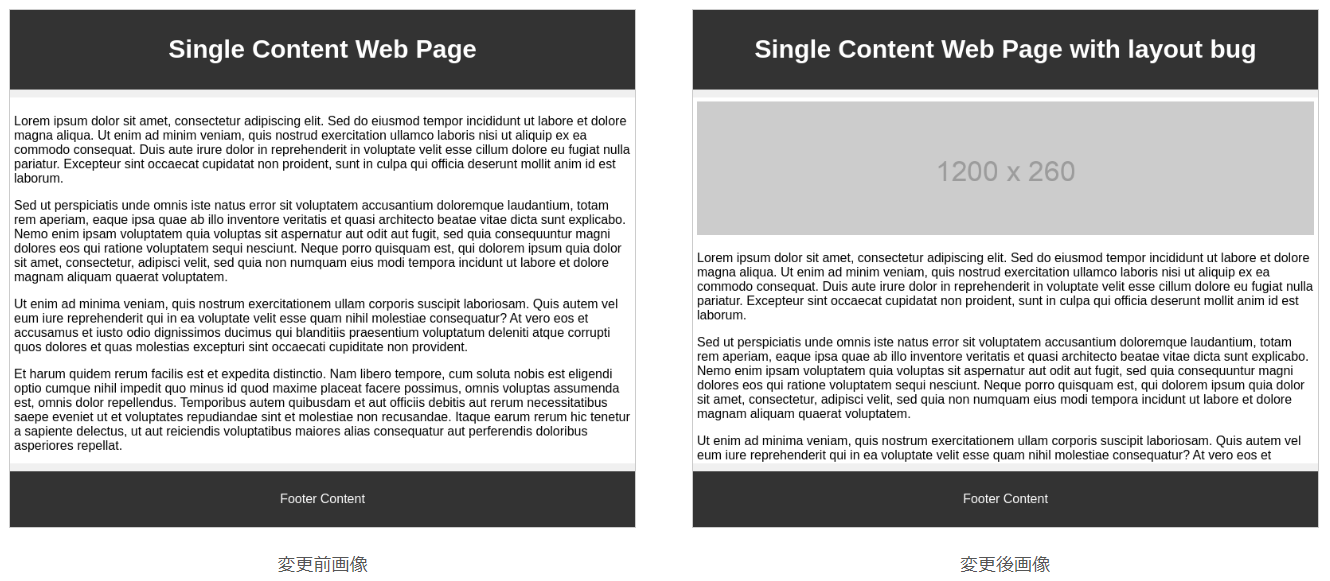
\includegraphics[width=1.0\columnwidth]{image/4_img_original_bf_af.png}
        \caption{\toolName のテスト対象とするWebページの変更前画像と変更後画像の例}
        \label{fig: img_original_bf_af}
    \end{center}
\end{figure}
以降、具体例に図\ref{fig: img_original_bf_af}を用いて、画像比較部の各処理について説明する。

\subsection{高解像度画像生成処理}\label{subsec:Generate_high_images}
高解像度画像生成処理は、図\ref{fig: img_original_bf_af}のWebページの変更前画像と変更後画像をそれぞれ高解像度画像にした、「変更前高解像度画像」と「変更後高解像度画像」を生成する。
「変更前高解像度画像」と「変更後高解像度画像」を、図\ref{fig: img_high_original_bf_af}に示す。
\begin{figure}[tp]
    \begin{center}
        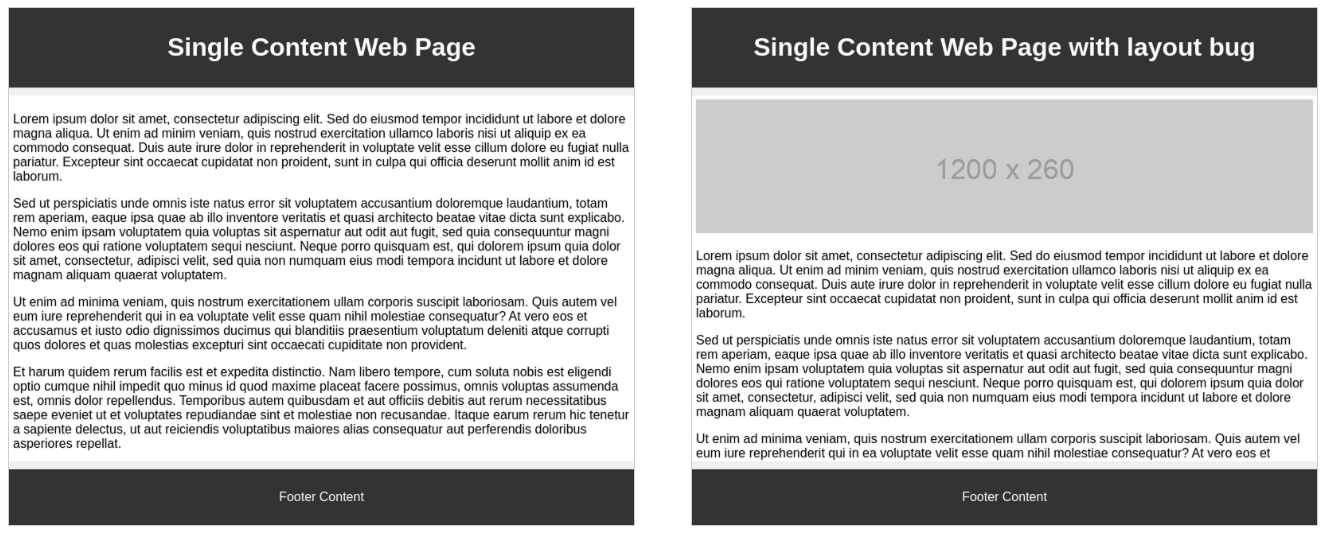
\includegraphics[width=1.0\columnwidth]{image/4_img_high_original_bf_af.png}
        \caption{「変更前高解像度画像」と「変更後高解像度画像」}
        \label{fig: img_high_original_bf_af}
    \end{center}
\end{figure}
この処理は、輪郭検出処理(\ref{subsec:contour_detection_processing}節で後述)の精度を向上するために必要である。
なお、生成した高解像度画像は他の処理部で使用するため、「変更前高解像度画像」と「変更後高解像度画像」をデータ管理部のbase\_dirディレクトリに出力する。
\par
高解像度画像を生成する流れを、以下に示す。なお、リサイズに使用するリサンプリングフィルタには、LANCZOSフィルタ(\ref{sec:pillow}節を参照)を用いる。
\begin{enumerate}
    \item PillowのImage.open関数(\ref{sec:pillow}節を参照)を用いて、Webページの画像パスから画像を読み込む。
    \item 画像の幅と高さを取得する。
    \item 画像の拡大率を設定する。本研究では、$2$とする。
    \item 画像のサイズ変更時に使用するリサンプリングフィルタを設定する。本研究では、PillowのImage.LANCZOSフィルタ(\ref{sec:pillow}節を参照)を用いる。
    \item Webページの画像を、画像の幅と高さにそれぞれ画像の拡大率を掛けたサイズの高解像度画像にリサイズする。
\end{enumerate}


\subsection{適応的二値化処理}\label{subsec:Adaptive_Binarisation}
適応的二値化処理は、図\ref{fig: img_high_original_bf_af}の「変更前高解像度画像」と「変更後高解像度画像」のそれぞれに対して、適応的二値化を行う。
この処理により、画像の一部が明るく、他の部分が暗い場合においても、全体として均一な二値化画像を生成できるため、
輪郭検出処理(\ref{subsec:contour_detection_processing}節で後述)の精度向上につながる。
処理の結果として、適応的二値化処理を行った、「変更前高解像度二値化画像」と「変更後高解像度二値化画像」を生成する。
「変更前高解像度二値化画像」と「変更後高解像度二値化画像」を、図\ref{fig: img_high_bin_bf_af}に示す。
\begin{figure}[tp]
    \begin{center}
        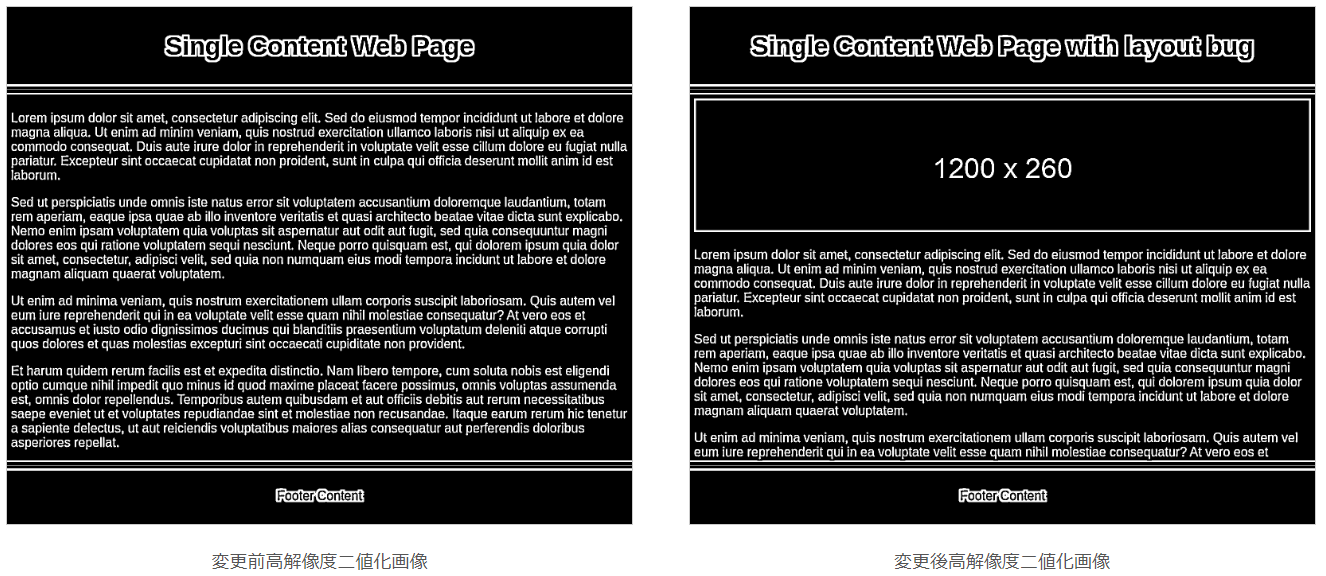
\includegraphics[width=1.0\columnwidth]{image/4_img_high_bin_bf_af.png}
        \caption{「変更前高解像度二値化画像」と「変更後高解像度二値化画像」}
        \label{fig: img_high_bin_bf_af}
    \end{center}
\end{figure}
\par
「変更前高解像度画像」と「変更後高解像度画像」に対して、それぞれ適応的二値化を行う流れを、以下に示す。
\begin{enumerate}
    \item OpenCVのimread関数(\ref{sec:opencv}節を参照)を用いて、画像を読み込む。
    \item OpenCVのcvtColor関数(\ref{sec:opencv}節を参照)を用いて、画像をグレースケール化する。
    \item OpenCVのadaptiveThreshold関数(\ref{sec:opencv}節を参照)を用いて、グレースケール画像に対して白黒反転を伴う適用的二値化を行う。
\end{enumerate}

\subsection{差分検出処理}\label{subsec:difference_detection_process}
差分検出処理は、図\ref{fig: img_high_bin_bf_af}の「変更前高解像度二値化画像」と「変更後高解像度二値化画像」に対して、差分検出を行う。
処理の結果として、Webページの変更前画像から削除された箇所と、Webページの変更後画像に追加された箇所をそれぞれ白い部分として可視化した、
「削除箇所二値化画像」と「追加箇所二値化画像」を生成する。
「削除箇所二値化画像」と「追加箇所二値化画像」を、図\ref{fig: img_del_add_bin_bf_af}に示す。
\begin{figure}[tp]
    \begin{center}
        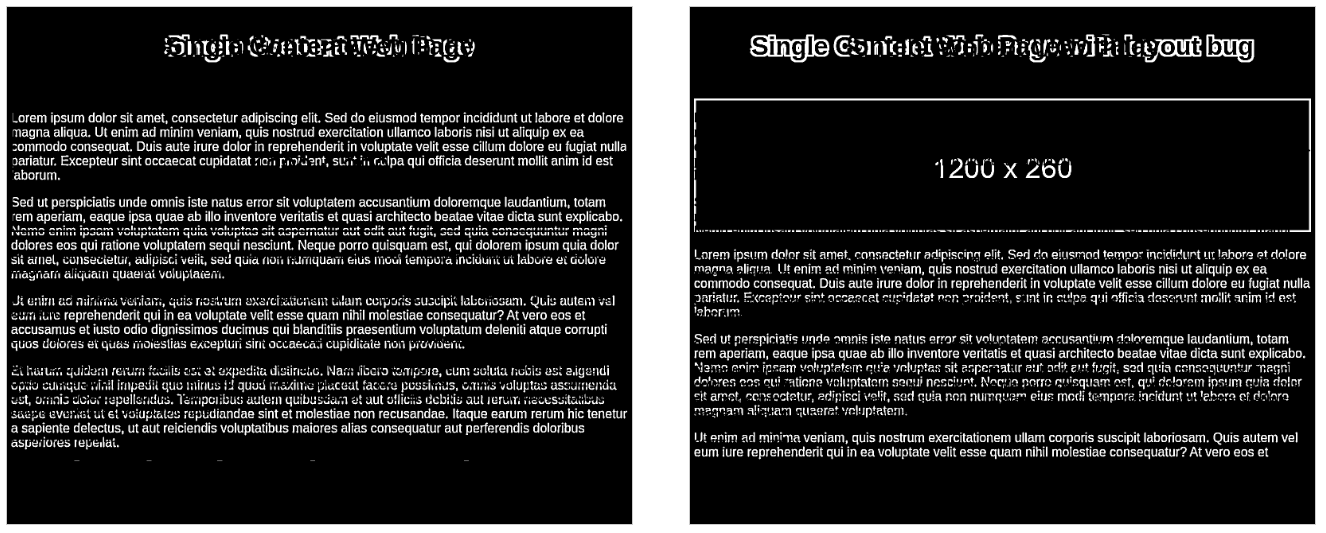
\includegraphics[width=1.0\columnwidth]{image/4_img_del_add_bin_bf_af.png}
        \caption{「削除箇所二値化画像」と「追加箇所二値化画像」}
        \label{fig: img_del_add_bin_bf_af}
    \end{center}
\end{figure}
図\ref{fig: img_del_add_bin_bf_af}を見ると、
図\ref{fig: img_high_bin_bf_af}の「変更前高解像度二値化画像」と「変更後高解像度二値化画像」を重ねたときの共通部分である白い箇所が消えており、
「変更前高解像度二値化画像」には、削除箇所が残り、「変更後高解像度二値化画像」には、追加箇所が残る。
これにより、輪郭検出処理(\ref{subsec:contour_detection_processing}節で後述)で、削除箇所を赤枠で、追加箇所を緑枠で囲むことができる。
\par
「変更前高解像度二値化画像」と「変更後高解像度二値化画像」に対して、差分検出処理を行う流れを、以下に示す。
\begin{enumerate}
    \item OpenCVのsubtract関数(\ref{sec:opencv}節を参照)の第一引数に「変更前高解像度二値化画像」を指定し、
          第二引数に「変更後高解像度二値化画像」を指定する。
    \item 1のsubtract関数によって、変更前の画像には存在するが変更後の画像には存在しない箇所を可視化した「削除箇所二値化画像」を生成する。
    \item subtract関数(\ref{sec:opencv}節を参照)の第一引数に「変更後高解像度二値化画像」を指定し、
          第二引数に「変更前高解像度二値化画像」を指定する。
    \item 3のsubtract関数によって、変更後の画像には存在するが変更前の画像には存在しない箇所を可視化した「追加箇所二値化画像」を生成する。
\end{enumerate}

\subsection{膨張処理}\label{subsec:dilation}
% (\ref{sec:dilation}節を参照)
膨張処理は、「削除箇所二値化画像」と「追加箇所二値化画像」のそれぞれの白い部分の形状とサイズを強調する。
この処理により、削除箇所と追加箇所の輪郭検出処理(\ref{subsec:contour_detection_processing}節で後述)を高める。
処理の結果として、膨張処理を行った、「削除箇所強調二値化画像」と「追加箇所強調二値化画像」を生成する。
「削除箇所強調二値化画像」と「追加箇所強調二値化画像」を、図\ref{fig: img_del_add_highlight_bin}に示す。
\begin{figure}[tp]
    \begin{center}
        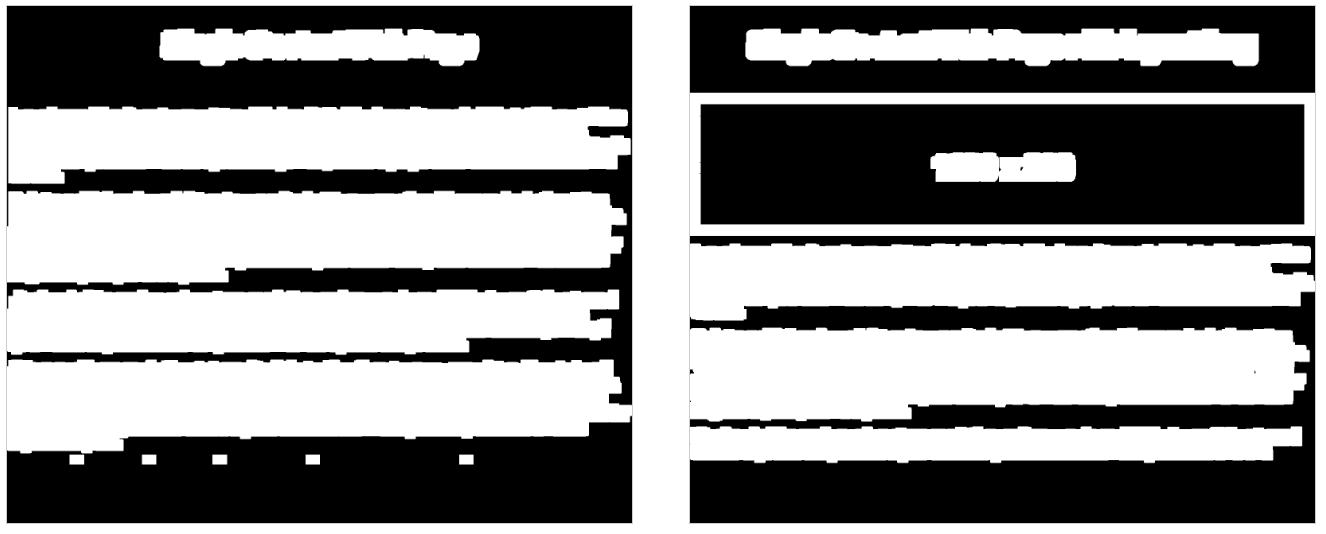
\includegraphics[width=1.0\columnwidth]{image/4_img_del_add_highlight_bin.png}
        \caption{「削除箇所強調二値化画像」と「追加箇所強調二値化画像」}
        \label{fig: img_del_add_highlight_bin}
    \end{center}
\end{figure}
\par
「削除箇所二値化画像」と「追加箇所二値化画像」に対して、膨張処理を適用する流れを、以下に示す。
\begin{enumerate}
    \item 特定の形状とサイズを持つカーネルを設定する。本研究では、5x5ピクセルの正方形カーネルを採用する。
    \item 設定したカーネルを用いて、膨張処理を適用する。適用後、画像内の削除箇所または追加箇所が拡大する。
    \item 2の膨張処理を複数回適用する。本研究では、膨張処理を6回繰り返すことで削除箇所または追加箇所を強調する。
    \item 膨張処理によって生成した「削除箇所強調二値化画像」と「追加箇所強調二値化画像」を輪郭検出処理に渡す。
\end{enumerate}

\subsection{輪郭検出処理}\label{subsec:contour_detection_processing}
輪郭検出処理は、OpenCVのfindContours関数(\ref{sec:opencv}節を参照)を用いて、図\ref{fig: img_del_add_highlight_bin}の「削除箇所強調二値化画像」と「追加箇所強調二値化画像」に対して、
削除箇所の輪郭と追加箇所の輪郭をそれぞれ検出する。
この処理の結果として、削除箇所の輪郭リストと追加箇所の輪郭リストを取得する。

\subsection{枠描画処理}\label{subsec:Bounding box drawing process}
枠描画処理は、Webページの変更前画像と変更後画像に対して、
輪郭検出処理(\ref{subsec:contour_detection_processing}節を参照)で取得した輪郭リストを用いて、
図\ref{fig: img_diff_highlight}に示した、
画像比較に基づく差分箇所を、色付きの枠で囲むことで強調表示した、Webページの変更前画像と変更後画像を生成する。
\begin{figure}[tp]
    \begin{center}
        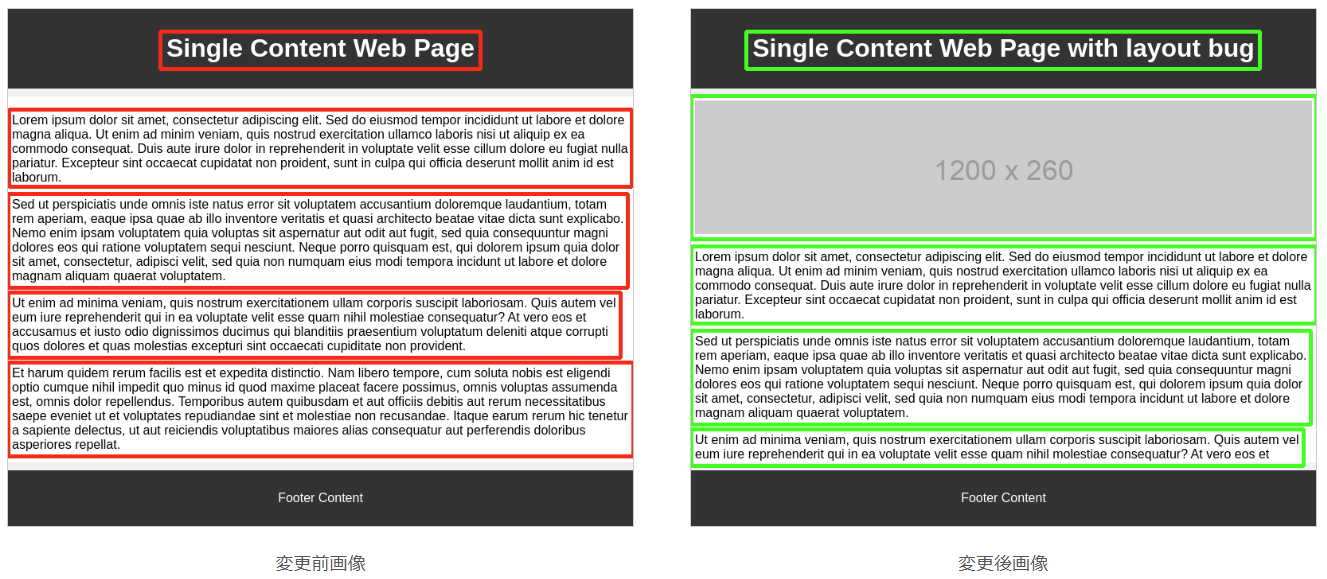
\includegraphics[width=1.0\columnwidth]{image/4_img_diff_highlight.png}
        \caption{画像比較に基づく差分箇所を、色付きの枠で囲むことで強調表示した、Webページの変更前画像と変更後画像}
        \label{fig: img_diff_highlight}
    \end{center}
\end{figure}
また、それらの画像から枠のみを残してそれ以外の部分を黒くすることで、差分箇所を囲む色付きの枠のみを抽出した、
「差分箇所赤枠強調マスク画像」と「差分箇所緑枠強調マスク画像」を生成する。
「差分箇所赤枠強調マスク画像」と「差分箇所緑枠強調マスク画像」を、図\ref{fig: img_diff_highlight_mask}に示す。
\begin{figure}[tp]
    \begin{center}
        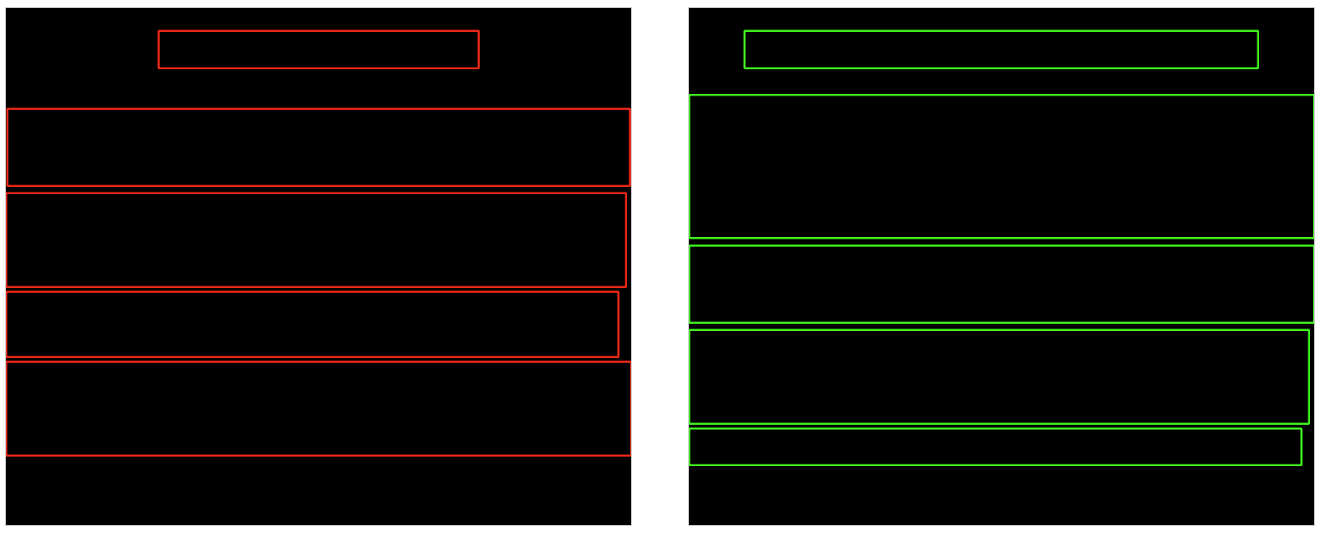
\includegraphics[width=1.0\columnwidth]{image/4_img_diff_highlight_mask.png}
        \caption{「差分箇所赤枠強調マスク画像」と「差分箇所緑枠強調マスク画像」}
        \label{fig: img_diff_highlight_mask}
    \end{center}
\end{figure}
\par
枠描画処理の流れを、以下に示す。
\begin{enumerate}
    \item cv2.boundingRect関数(\ref{sec:opencv}節を参照)を用いて、輪郭リストの各要素である輪郭データから、輪郭を囲む矩形の座標と幅、高さを取得する。
    \item 取得した矩形情報を引数に指定したcv2.rectangle関数(\ref{sec:opencv}節を参照)を用いて、Webページの変更前画像上に赤枠、Webページの変更後画像上に緑枠を描画する。
    \item np.zeros関数(\ref{sec:numpy}節を参照)を用いて、Webページの変更前画像と変更後画像のそれぞれと同じサイズの黒画像を生成する。
    \item 取得した矩形情報を引数に指定したcv2.rectangle関数を用いて、生成した2つの黒画像に対して、一方の黒画像には赤枠を、もう一方の黒画像には緑枠を描画する。
\end{enumerate}


%%%% HTML比較 %%%%
% 画像比較部は、データ管理部のbase\_dirディレクトリからWebページの変更前画像と変更後画像を受け取り、
% 画像比較に基づく差分箇所を色付きの枠で囲むことで強調表示したWebページの変更前画像と変更後画像を生成する。
% また、それらの画像から枠のみを残してそれ以外の部分を黒くすることで、差分箇所を囲む色付きの枠のみを抽出した、「差分箇所赤枠強調マスク画像」と「差分箇所緑枠強調マスク画像」も生成する。
% 生成した画像は、データ管理部のbase\_dirディレクトリに出力する。
% \par
% 画像比較部の処理の流れを、以下に示す。
% \begin{enumerate}
%     \item 高解像度画像生成処理
%     \item 適応的二値化処理
%     \item 差分検出処理
%     \item 膨張処理
%     \item 輪郭検出処理
%     \item 枠描画処理
% \end{enumerate}
% また、\toolName のテスト対象とするWebページの変更前画像と変更後画像の例を、図\ref{fig: img_original_bf_af}に示す。
% \begin{figure}[tp]
%     \begin{center}
%         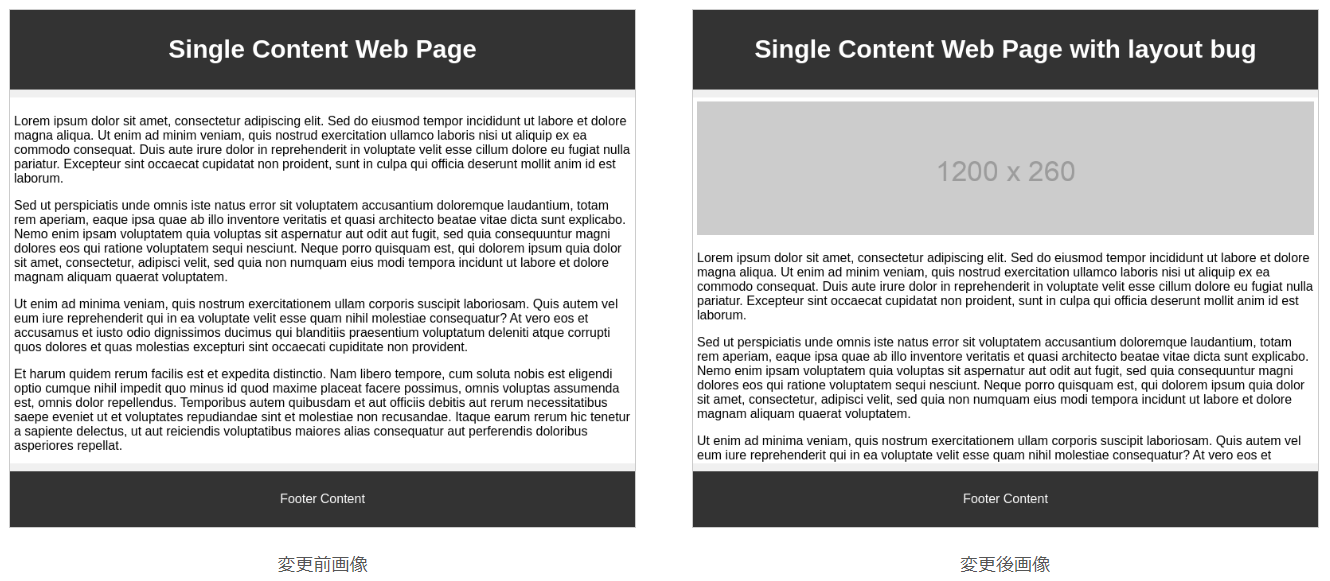
\includegraphics[width=1.0\columnwidth]{image/4_img_original_bf_af.png}
%         \caption{\toolName のテスト対象とするWebページの変更前画像と変更後画像の例}
%         \label{fig: img_original_bf_af}
%     \end{center}
% \end{figure}
% 以降、具体例に図\ref{fig: img_original_bf_af}を用いて、画像比較部の各処理について説明する。
\section{HTML比較部}\label{sec:Affected_area_extraction}
HTML比較部は、データ管理部のbase\_dirディレクトリからWebページの変更前HTMLコードと変更後HTMLコードを受け取り、
HTMLコードの変更に基づく影響箇所を色付きの枠で囲むことで強調表示した、Webページの変更前画像と変更後画像を生成する。
また、それらの画像から枠のみを残してそれ以外の部分を黒くすることで、影響箇所を囲む色付きの枠のみを抽出した、「影響箇所赤枠強調マスク画像」と「影響箇所緑枠強調マスク画像」も生成する。
生成した画像は、データ管理部のbase\_dirディレクトリに出力する。
\par
HTML比較部の処理の流れを、以下に示す。
\begin{enumerate}
    \item 差分コード生成処理
    \item 差分コード解析処理
    \item 影響箇所強調HTMLコード生成処理
    \item 枠抽出処理
\end{enumerate}
以降、図\ref{fig: img_original_bf_af}の例で挙げたWebページの、変更前HTMLコードと変更後HTMLコードを具体例に、
HTML比較部の各処理について説明する。

\subsection{差分コード生成処理}\label{subsec:diff_file_generate}
差分コード生成処理は、Webページの変更前HTMLコードと変更後HTMLコードを行ごとに比較して、txt形式の差分コードを生成する。
生成したtxt形式の差分コードの例を、ソースコード\ref{lst:diff_html}に示す。
ソースコード\ref{lst:diff_html}の3行目を見ると、先頭に"-"が付いており、この行は削除行であることを示す。
また、ソースコード\ref{lst:diff_html}の4行目および8行目を見ると、先頭に"+"が付いており、この行は追加行であることを示す。
このように、生成したtxt形式の差分コードには、コードの追加行の先頭に"+"、削除行の先頭に"-"を付加する。
\begin{figure}[tp]
    \begin{lstlisting}[language=HTML, caption=生成したtxt形式の差分コードの例, label=lst:diff_html]
<body>
    <header>
-         <h1>Single Content Web Page</h1>
+         <h1>Single Content Web Page with layout bug</h1>
    </header>
    <div class="container">
        <div class="main-content">
+             <img src="https://via.placeholder.com/1200x260" alt="Placeholder Image">
              // テキスト文省略
        </div>
    </div>
    <footer>
        <p>Footer Content</p>
    </footer>
</body>
    \end{lstlisting}
\end{figure}
\par
差分コードを生成する処理を、以下に示す。
\begin{enumerate}
    \item 変更前HTMLコードと変更後HTMLコードをそれぞれHTMLデータとして読み込む。
    \item HTMLデータ内の$<$p$>$タグ内のテキスト内に存在する余分な空白や改行を取り除く(\ref{sec:text_change}節を参照)ために、以下を行う。
          \begin{enumerate}
              \item 変更前と変更後のHTMLデータを解析するためのBeautifulSoupオブジェクト(\ref{sec:beautifulsoup}節を参照)をそれぞれ初期化する。
              \item BeautifulSoupオブジェクトに対して、find\_all関数(\ref{sec:beautifulsoup}節を参照)を用い、HTMLデータ内の全ての$<$p$>$タグを格納したリストを生成する。
              \item get\_text関数(\ref{sec:beautifulsoup}節を参照)を用いて、生成したリストの各要素内における$<$p$>$タグのテキストを取得する。
              \item Pythonの文字列関数であるsplit関数を用いて、取得した各テキストを空白文字で分割する。
              \item Pythonの文字列関数であるjoin関数を用いて、分割したテキストを再び空白文字で連結する。
              \item BeautifulSoupオブジェクトをstring型に変換し、HTMLデータ形式に戻す。
          \end{enumerate}
    \item difflib(\ref{sec:difflib}節を参照)のDifferクラスとcompare関数を用いて、2つのHTMLデータ間を行ごとに比較し、差分コードを生成する。
    \item 生成した差分コードから、行の先頭が"?"から始まる行を除外する。
    \item 差分コードをtxt形式で保存する。
\end{enumerate}

% \subsection{差分コード解析処理}\label{subsec:diff_file_analyze}
% 差分コード解析処理は、差分コード生成処理から差分コードを受け取り、差分コードからbody要素内の変更箇所とstyle要素内の変更箇所を検出する。
% \par
% 差分コードを解析する処理を、以下に示す。

% 枠付きHTMLコード生成するためには、以下の処理を行う。
% body要素内の変更箇所を検出する。
% 差分コードの先頭の行に対して、以下の処理を行う。
% 1.body要素外であるか判定する。body要素外ならば、以下の処理を行う。
% 1. 先頭行が"-"であれば、
% body要素内の各先頭行に"+"または"-"がある箇所を探す。
% "+"や"-"であれば、その行に対して以下の操作を行う。
% 1."+"または"-"を削除する。
% 2.行にimgタグが含まれている場合、img用の枠を囲むCSSクラスを追加する。
% 3.行にimgタグが含まれていない場合、行中に開始タグが存在するかを確認する。
% 4.行中に開始タグが存在する場合は、タグ内にclass属性が既にあるかどうか確認する。行中に開始タグが存在しない場合は、何もしない。
% 5.class属性があれば、class=""の中の末尾に枠をつけるクラスを追加する。
% 6.class属性が無ければ、終了タグ直前に枠をつけるクラスを追加する。

% body要素内の変更箇所に枠をつけるCSSクラスを追加する。
% style要素内の変更箇所を検出する。
% style要素内の変更箇所に枠をつけるCSSクラスを追加する。

\subsection{枠付きHTMLコード生成処理}\label{subsec:modified_html_generate}
【TODO: 処理を整理する必要あり】\\
枠付きHTMLコード生成処理は、差分コード生成処理から差分コードを受け取り、枠付き変更前HTMLコードと枠付き変更後HTMLコードを生成する。
なお、枠付き変更前HTMLコードは、影響箇所(\ref{cha:Function}を参照)における削除箇所に赤枠をつけるCSSクラスを付与した、変更前HTMLコードと定義する。
また、枠付き変更後HTMLコードは、影響箇所における追加箇所に緑枠をつけるCSSクラスを付与した、変更後HTMLコードと定義する。
\par
差分コードから、枠付き変更前HTMLコードと枠付き変更後HTMLコードを生成する処理を、以下に示す。
\begin{enumerate}
    \item CSSセレクタ抽出処理
    \item body要素解析処理
    \item CSSクラス定義処理
\end{enumerate}

\subsubsection{CSSセレクタ抽出処理}\label{subsubsec: style_analysis}
CSSセレクタ抽出処理は、style要素内において変更があったCSSセレクタ\cite{CssSelector}を、差分コードから全て抽出する。
抽出したCSSセレクタは、リストにそれぞれ格納し、CSSクラス定義処理(\ref{subsubsec: css_define}節に後述)に出力する。
sytle要素解析処理の流れを、以下に示す。
\begin{enumerate}
    \item 変更があったCSSセレクタを格納するリストであるchanged\_selectorsを、空リストとして初期化する。
    \item 現在処理中のCSSセレクタを保持するための変数であるcurrent\_selectorの値を、Noneに初期化する。
    \item 差分コードの全ての行に対して、先頭行から順に1行ずつ文字列の判定をし、判定結果に応じて、以下の処理を行う。
          \begin{enumerate}
              \item CSSセレクタの開始を示す"\{"を含む行を見つけた場合:
                    \begin{enumerate}
                        \item 行中のCSSセレクタのみを抽出する。
                        \item changed\_selectors内に抽出したセレクタが存在せず、かつ、行が変更を示す"+"、または、"-"で始まる場合、
                              CSSセレクタをchanged\_selectorsに格納する。
                        \item current\_selectorの値にCSSセレクタを格納し、現在処理中のCSSセレクタを更新する。
                    \end{enumerate}
              \item CSSセレクタの終了を示す"\}"を含む行を見つけた場合:
                    \begin{enumerate}
                        \item current\_selectorの値にNoneを格納し、現在処理中のCSSセレクタをリセットする。
                        \item 3に戻る。
                    \end{enumerate}
              \item current\_selectorの値にCSSセレクタが格納されており、行が変更を示す"+"、または、"-"で始まる場合:
                    \begin{enumerate}
                        \item changed\_selectors内に、current\_selectorに格納されているCSSセレクタが存在しないならば、
                              そのCSSセレクタをchanged\_selectorsに格納する。
                    \end{enumerate}
          \end{enumerate}
    \item changed\_selectorsをCSSクラス定義処理に出力する。
\end{enumerate}

\subsubsection{body要素解析処理}\label{subsubsec: body_analysis}
body要素解析処理は、変更前後のWebページでbody要素内に変更があったタグ要素のstyle属性にCSSクラスを付与しつつ、
枠付き変更前HTMLコードと枠付き変更後HTMLコードを生成する中間の処理を行う。
body要素解析処理の流れを、以下に示す。
なお、枠付き変更前HTMLコードの各行を格納するリストmodified\_before\_linesと枠付き変更後HTMLコードの各行を格納するリストmodified\_after\_linesを空リストとして初期化する。
また、処理を行う行が削除行であると判定する変数flag\_beforeと追加行であると判定する変数flag\_afterをそれぞれFalseで初期化する。
さらに、差分コードの先頭行から順に各行に対して、以下の処理を行うものとする。
\begin{enumerate}
    \item 行がbody要素外の場合:
          \begin{enumerate}
              \item 行の先頭が"-"の場合、modified\_before\_linesに行を追加する。
              \item 行の先頭が"+"の場合、modified\_after\_linesに行を追加する。
              \item 行の先頭がそれ以外の場合、modified\_before\_linesとmodified\_after\_linesの両方に行を追加する。
          \end{enumerate}
    \item 行がbody要素内の場合:
          \begin{enumerate}
              \item (b)と(c)はif-elseブロック
              \item 行の先頭が"-"または"+"の場合:
                    \begin{enumerate}
                        \item 行の先頭が"-"の場合、flag\_beforeの値をTrueにし、"-"を取り除く
                        \item 行の先頭が"+"の場合、flag\_afterの値をTrueにし、"+"を取り除く
                        \item 行中に"\textless img"を含む場合:
                              \begin{enumerate}
                                  \item imgタグ用のCSSクラスを付与したdivタグでimgタグを囲む。
                              \end{enumerate}
                        \item 行中に"\textless img"を含まない場合:
                              \begin{enumerate}
                                  \item 行中に"class="を含む場合、開始タグのstyle属性にbody要素用のCSSクラスを付与する。
                                  \item 行中に"class="を含まない場合、開始タグの終了記号直前にbody要素用のCSSクラスを付与する。
                              \end{enumerate}
                    \end{enumerate}
              \item 行の先頭がそれ以外の場合:\\
                    flag\_beforeとflag\_afterの両方の値をFalseにする。
              \item (e)と(f)と(g)はif-elif-elseブロック
              \item flag\_beforeの値がTrue、 かつ、flag\_afterの値がFalseの場合、modified\_before\_linesに行を追加する。
              \item flag\_beforeの値がFalse、 かつ、flag\_afterの値がTrueの場合、modified\_after\_linesに行を追加する。
              \item それ以外の場合、modified\_before\_linesとmodified\_after\_linesの両方に行を追加する。
          \end{enumerate}
\end{enumerate}

\subsubsection{CSSクラス定義処理}\label{subsubsec: css_define}
CSSクラス定義処理は、body要素解析処理から未完成の枠付き変更前HTMLコードと枠付き変更後HTMLコードのそれぞれに対して、
style要素内の末尾にCSSクラスの定義を追記する。
【TODO: 処理内容を書く】

\subsection{枠抽出処理}\label{subsec:frame_extraction}
枠抽出処理は、Webページの変更前画像と枠付きを行ったWebページの変更前画像を比較し、赤枠のみを抽出した画像を生成する。
また、Webページの変更後画像と枠付きを行ったWebページの変更後画像を比較し、緑枠のみを抽出した画像を生成する。
生成した画像は、レイアウトの副作用抽出部に出力する。
\par
枠抽出処理の流れを、以下に示す。
\begin{enumerate}
    \item 枠付きHTMLコードをローカルサーバ上(\ref{sec:Flask}節を参照)でWebページとして公開する
    \item 取得部を用いて、枠付きHTMLコードをもとにしたWebページの画像を取得する
    \item Webページの変更前画像と枠付きを行ったWebページの変更前画像を比較し、赤枠のみを抽出した変更前画像を生成する
    \item Webページの変更後画像と枠付きを行ったWebページの変更後画像を比較し、緑枠のみを抽出した変更後画像を生成する
\end{enumerate}

% \section{影響箇所検出部}\label{sec:Affected_area_extraction}
% HTMLコードの変更に基づく影響箇所抽出部は、Webページ情報取得部で取得した変更前後のWebページのHTMLコードを用いて影響箇所を特定する。
% 概要としては、差分コードを生成し、差分コードから枠付き処理を行った変更前後のHTMLコードを生成した後、そのHTMLコードをFlaskのテンプレートエンジンを用いてWebページを表示し、Webページ情報取得部によってそのWebページの画像を取得する。
% 元のWebページ画像と枠付き処理をしたWebページ画像を比較して枠のみを抽出する。
% 具体的には、まず、Pythonライブラリの一つであるdifflibモジュールを用いて、変更前後のHTMLコードから差分コードを生成する。
% 生成した差分コードは、コードの追加行には"+", 削除行には"-", 変更前後のHTMLコードにどちらにも存在しない行には"?"が先頭に付き、"?"を除いた差分コードを解析対象とする。
% 差分コードは、bodyタグ内とstyleタグ内を対象とする。
% もし、bodyタグ内で先頭に"+"や"-"があれば、コードの追加や削除、変更があったとして、その箇所に枠付き処理を行うCSSクラスを追加し、先頭の"+"か"-"を削除する。
% styleタグ内の場合は、CSSクラスのセレクタ名のみの変更やスタイルのみの変更、またはその両方の変更があったCSSクラスを対象として、そのCSSクラスに対して枠付きを行うスタイルを適用する。
% この場合においても、解析した行の先頭に"+", "-"があれば削除する。
% 差分コードから枠付き処理を行った変更前後のHTMLコードを生成した後は、そのHTMLコードをFlaskのテンプレートエンジンを用いてWebページとして表示し、そのWebページの画像を取得する。
% そして、元のWebページ画像と枠付き処理をしたWebページ画像を比較して枠のみを抽出する。
\section{副作用抽出部}\label{sec:Layout_subEffect_extraction_section}
副作用抽出部は、データ管理部のdiff\_dirディレクトリから「差分箇所赤枠強調マスク画像」と「差分箇所緑枠強調マスク画像」、「影響箇所赤枠強調マスク画像」と「影響箇所緑枠強調マスク画像」を受け取り、
これらの画像から、レイアウトの副作用箇所を抽出した、変更前画像と変更後画像を生成する。
生成した画像は、データ管理部のdiff\_dirディレクトリに出力する。
副作用抽出部の処理の流れを、以下に示す。
\begin{enumerate}
    \item 「差分箇所赤枠強調マスク画像」と「影響箇所赤枠強調マスク画像」をcv2.imread関数で読み込む。
    \item cvtColor関数でグレースケール化する。
    \item threshold関数で二値化を行う。
    \item 二値化した「差分箇所赤枠強調マスク画像」に対して、cv2.findContours関数で輪郭リストcontours\_img\_bfを取得する。
    \item 二値化した「影響箇所赤枠強調マスク画像」に対して、cv2.findContours関数で輪郭リストcontours\_html\_bfを取得する。
    \item contours\_img\_bfの各輪郭要素の数だけループして、以下の処理を行う。
          \begin{enumerate}
              \item contours\_html\_bfの各輪郭要素の数だけループして、以下の処理を行う。
                    \begin{enumerate}
                        \item  contours\_img\_bfとcontours\_html\_bfのそれぞれの輪郭要素のバウンディングボックスを取得する。
                        \item バウンディングボックスが重なっているか判定する
                              \begin{enumerate}
                                  \item  重なっている場合は、重なり部分のバウンディングボックスの面積を計算する。
                                        小さい方のバウンディングボックスの面積を計算する。
                                        重なり部分のバウンディングボックスの面積が、小さい方のバウンディングボックスの面積の6割を超えれば、
                                        大きい方のバウンディングボックスと小さい方のバウンディングボックスが重なっていると判定し、Trueを返す。そうでなければ、Falseを返す。
                                  \item 重なっていない場合は、Falseを返す。
                              \end{enumerate}
                    \end{enumerate}
              \item matchの値がTrueなら、ループ処理から抜ける。
          \end{enumerate}
    \item matchの値がTrueなら、contours\_img\_bfの輪郭要素をunique\_contours\_bfに格納する。
    \item 「差分箇所緑枠強調マスク画像」上の各緑枠と「影響箇所赤枠強調マスク画像」上の各緑枠を比較する。
\end{enumerate}
% レイアウトの副作用抽出部は、画像比較に基づく差分箇所とHTMLコードの変更に基づく影響箇所を用いて、レイアウトの副作用箇所を抽出する。
% 具体的には、差分箇所を囲む枠と影響箇所を囲む枠同士を比較する。比較の仕方は、枠の重なり度合を判定する。
% まず、枠が重なっているかどうかを判定する。次に、枠が重なっている場合に、重なり部分が小さい方の枠の面積の6割以上であれば枠が一致すると判定する。
% 最終的に、一致しない枠のみを抽出し、一致しない赤枠をWebページの変更前画像に、一致しない緑枠をWebページの変更後画像に描画し、保存する。
% 「」と「」を、図\ref{fig: subeffect_name}に示す。
\begin{figure}[tp]
    \begin{center}
        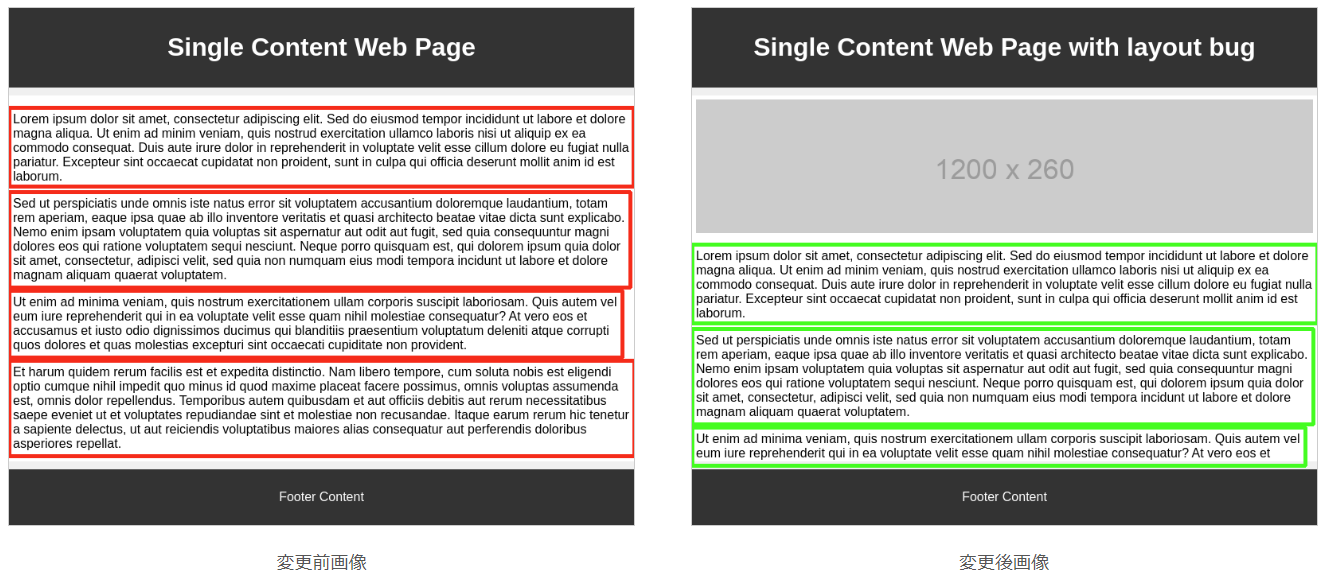
\includegraphics[width=1.0\columnwidth]{image/4_subeffect_name.png}
        \caption{レイアウト副作用箇所を色付きの枠で囲むことで強調表示した、変更前画像と変更後画像}
        \label{fig: subeffect_name}
    \end{center}
\end{figure}
\par

\section{不具合抽出部}\label{sec:Layout_bug_extraction_section}
レイアウト不具合抽出部は、データ管理部のdiff\_dirディレクトリから~画像を受け取り、
副作用抽出部から抽出したレイアウトの副作用箇所から、レイアウトの不具合箇所を抽出する。
具体的には、\ref{sec:Layout_subEffect_extraction_section}節で抽出したレイアウトの副作用箇所を囲んだ各赤枠内の領域と、レイアウトの副作用箇所を囲んだ各緑枠内の領域を比較する。
その後、赤枠内の領域と緑枠内の領域をabsdiff関数(\ref{sec:opencv}節を参照)で絶対差分を計算して類似度を求める。
類似度が9割を超えれば、レイアウトの不具合は無いと判定し、比較した赤枠と緑枠を除外する。
上記の処理によって、類似度が9割未満であった赤枠と緑枠を抽出することができ、それらはレイアウトの不具合として、Webページの変更前画像と変更後画像に描画する。
\begin{enumerate}
    \item 「差分箇所赤枠強調マスク画像」と「影響箇所赤枠強調マスク画像」をcv2.imread関数で読み込む。
    \item cvtColor関数でグレースケール化する。
    \item threshold関数で二値化を行う。
    \item 二値化した「差分箇所赤枠強調マスク画像」に対して、cv2.findContours関数で輪郭リストcontours\_img\_bfを取得する。
    \item 二値化した「影響箇所赤枠強調マスク画像」に対して、cv2.findContours関数で輪郭リストcontours\_html\_bfを取得する。
    \item contours\_img\_bfの各輪郭要素の数だけループして、以下の処理を行う。
          \begin{enumerate}
              \item contours\_html\_bfの各輪郭要素の数だけループして、以下の処理を行う。
                    \begin{enumerate}
                        \item 領域間の類似度を計算する。
                    \end{enumerate}
          \end{enumerate}
    \item 
    \item 「差分箇所緑枠強調マスク画像」上の各緑枠と「影響箇所赤枠強調マスク画像」上の各緑枠を比較する。
\end{enumerate}

\section{表示部}\label{sec:Interface_Display_Section}
表示部は、データ管理部のdiff\_dirディレクトリ内にある
\ref{sec:Web_data_get_section}節~\ref{sec:Layout_bug_extraction_section}節で取得・生成した画像(枠強調マスク画像を除く)を受け取り、
Webベースのinterfaceユーザを用いて表示する。
MixVRTの実行コマンド初回実行時は、\ref{sec:Web_data_get_section}節で取得したWebページの画像を表示する。
MixVRTの実行コマンド2回目以降実行時は、初回実行時に取得する画像に加えて、\ref{sec:Difference_extraction_section}節で取得した画像、
\ref{sec:Affected_area_extraction}節で生成した画像、\ref{sec:Layout_bug_extraction_section}節で生成した画像を表示する。
